\documentclass[12pt,a4paper]{article}
\usepackage{geometry}
\usepackage{wrapfig}
\usepackage[utf8]{inputenc}
\usepackage[english]{babel}
\usepackage{titlesec}
\usepackage{graphicx}
\usepackage{subfigure}

\titlespacing*{\section}
{0pt}{2ex minus .2ex}{2ex plus .2ex}
\titlespacing*{\subsection}
{0pt}{1ex minus .2ex}{1ex plus .2ex}

\setlength{\parindent}{2em}
\setlength{\parskip}{0.5em}

\title{\vspace{-2cm}Assignment3 Report\vspace{-2ex}}
\author{Wang Youan (3035237236)\\ MSc in Computer Science, the University of Hong Kong\vspace{-2ex}}
\date{\today\vspace{-1cm}}
\graphicspath{{images/}}
\geometry{left=2cm, right=2cm, top=2cm, bottom=2cm}
\begin{document}
	\maketitle
	\section{Markov Decision Processes}
	\subsection{Value Iteration Agent}
	I use $ Q_{k+1}(s,a)=\sum_s' P(s' | s, a) (R(s,a,s')+\gamma V_k(s')) $ and $ V_k(s)=\max_aQ_k(s,a) $ to update Q-values\par
	In the typical grid world, this algorithm will be convergence after about 31 iterations (the absolute different value is less than 1e-8) seems not so bad.
	\subsection{BridgeGrid}
	The are two ways to let the agent choose a far exit with large credit, one is increase discount factor, the other one is decrease noise factor. About this question, the discount factor is large enough, thus we need to change the noise level.\par
	Final in the leftmost cell, Q-value of going left is $ 0.9 - 90.9\gamma $, going right is approximately $ 5.9049 - 398.0835\gamma + 718.875\gamma^2 - 683.073\gamma^3 $. We should make sure that $ 5.9049 - 398.0835\gamma + 718.875\gamma^2 - 683.073\gamma^3 > 0.9 - 90.9\gamma $, which means that, $ \gamma < 0.016955 $. In the answer.py, I put 0.016954, which will also pass this question
	\subsection{DiscountGrid}
	The principle to solve this grid is that, 
	\begin{enumerate}
		\vspace{-2ex}\item Agent with larger discount factor prefers the distant exit(+10), and vice verse
		\vspace{-1ex}\item Agent with larger noise factor will avoid the cliff, and less one will risk the cliff
		\vspace{-1ex}\item If living reward is large enough, agent will avoid both exits and the cliff, so as to get the infinite living reward.
	\end{enumerate}
	\vspace{-2ex}Based on the above three principles, the question is easy to answer.
	\section{Q-learning}
	\subsection{Q-learning Agent}
	The formula of Q-learning agent is similar to that of a value iteration agent, but the their usages are totally different. The learning process of Q-learning agent is based on experience, and can not full observed environment. That means such type of agent is much closer to reality.\par
	Using such method, crawler will need almost half an hour to find the best solution, takes 10000 steps to learn, which sounds very cost and slow. However, it takes human beings much longer to have nowadays level. The learning process of crawler looks as if human growth process.
	\subsection{BridgeGrid}
	My answer to this question is \textbf{impossible}.\par
	In this noiseless world, to achieve the distant exit with +10 needs 5 steps, which means that even if set the epsilon to 0, i.e. a total stochastic world, there is only $ \frac{1}{4}^5 \approx 0.098\% $ chance to reach that cell. With just 50 tries, it is impossible to have enough chance to evaluate the value. There should at least 10000 epsilon total stochastic tries. For a partial random agent (whose epsilon is larger than 0), the chance of learning best policy is much lower.\par
	This question shows one shortage of Q-learning agent that as it lacks the overview of global environment, it may not find the optimal solutions. 
	\section{Approximate Q-learning and State Abstraction}
	\subsection{Q-learning Agent}
	Q-learning agent is a bad learner in Pacman, even for middle grid. The reasons are 
	\begin{itemize}
		\vspace{-2ex}\item Because of lacking the ability of abstraction, q-learning agent will regard two similar state (e.g. figure~\ref{fig:smilar}, actually these two states are almost the same) as totally different one. (e.g, two states whose only differences are the food number)
		\begin{figure}[ht]
			\centering
			\subfigure[State A]{
				\centering
				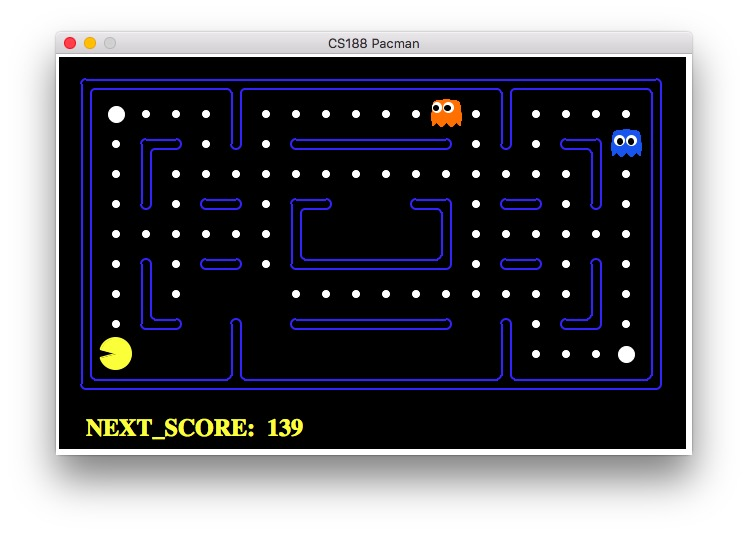
\includegraphics[width=.4\linewidth]{state_a}
			}
			\subfigure[State B]{
				\centering
				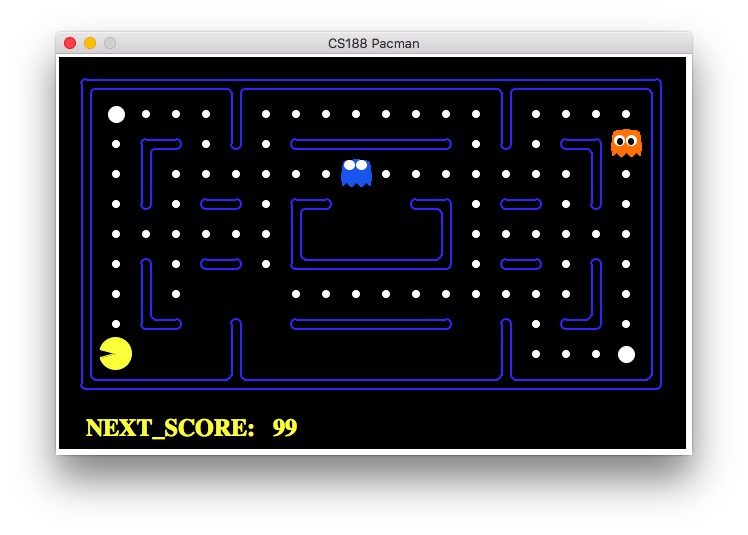
\includegraphics[width=.4\linewidth]{state_b}
			}
			\caption{Two similar states}
			\label{fig:smilar}
		\end{figure} 
		\vspace{-2ex}\item Because of randomness. Q-learning agent makes stochastic action, sometimes it will return some totally unreasonable direction, such as rushing to the Ghost.
	\end{itemize}
	\vspace{-2ex}One strong point of Q-learning algorithm is that we don't need any knowledge about the environment. Such type of agent can learn everything from there own actions. However, lacking pre-knowledge is also its shortcoming, which makes Q-learning algorithm not suitable for such type of problems with many similar states and we have some experience. We have to try other methods. 
	\subsection{Approximate Q-learning Agent}
	In order to address deficiencies of Q-learning algorithm, we will combine our learning agent with some special knowledge. The biggest difference between the two methods is that approximate Q-leaning agent uses feature-based model instead state-based one in Q-learning agent.\par
	We can easily solve middleClassic grid with only 50 episodes with proper design feature extractor.
\end{document}